\def\iangle{35} % Angle of the inclined plane
\def\down{0}
\def\arcr{0.7cm} % Radius of the arc used to indicate angles
\newcommand\centerofmass{%
    \tikz[radius=0.2em] {%
        \fill (0,0) -- ++(0.2em,0) arc [start angle=0,end angle=90] -- ++(0,-0.4em) arc [start angle=270, end angle=180];%
        \draw (0,0) circle;%
    }%
}

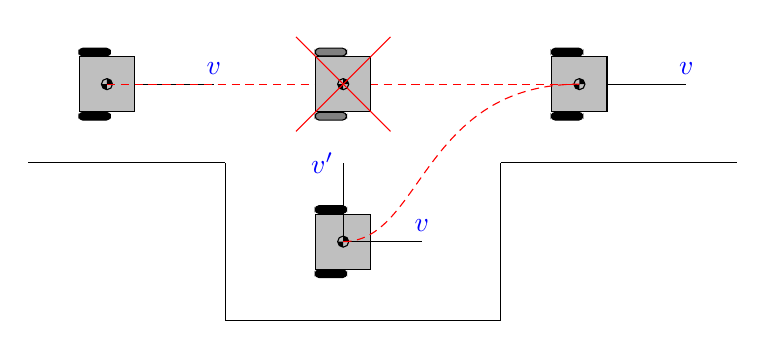
\begin{tikzpicture}[
    force/.style={>=latex,draw=blue,fill=blue},
    axis/.style={densely dashed,gray,font=\small},
    M/.style={rectangle,draw,fill=lightgray,minimum size=0.7cm,thin},
    m/.style={rectangle,draw=black,fill=lightgray,minimum size=0.3cm,thin},
    plane/.style={draw=black,fill=blue!10},
    string/.style={draw=red, thick},
    pulley/.style={thick},
    wheel/.style={fill=black, rounded corners=1.5pt},
]
     \begin{scope}[rotate=0]
        \node[M,transform shape] (M1) at (0,0) {\centerofmass};
        % Draw axes and help lines
        % Forces
        {[force,->]
            % Assuming that Mg = 1. The normal force will therefore be cos(alpha)
            \draw (M1.east) -- ++(1,0) node[above, blue] {$v$};
        }

        \draw[wheel,] (M1.south west) rectangle ++(.4,-.1) node[]{};
        \draw[wheel,] (M1.north west) rectangle ++(.4,.1)  node[]{};
    \end{scope}


    \begin{scope}[rotate=0]
        \node[M,transform shape] (M2) at (6,0) {\centerofmass};
        % Draw axes and help lines
        % Forces
        {[force,->]
            % Assuming that Mg = 1. The normal force will therefore be cos(alpha)
            \draw (M2.east) -- ++(1,0) node[above, blue] {$v$};
        }

        \draw[wheel,] (M2.south west) rectangle ++(.4,-.1) node[]{};
        \draw[wheel,] (M2.north west) rectangle ++(.4,.1)  node[]{};
    \end{scope}
    \begin{scope}[rotate=0]
        \node[M,transform shape] (M3) at (3,-2) {\centerofmass};
        % Draw axes and help lines
        % Forces
        {[force,->]
            % Assuming that Mg = 1. The normal force will therefore be cos(alpha)
            \draw (M3.center) -- ++(1,0) node[above, blue] {$v$};
            \draw (M3.center) -- ++(0,1) node[left, blue] {$v'$};
        }

        \draw[wheel,] (M3.south west) rectangle ++(.4,-.1) node[]{};
        \draw[wheel,] (M3.north west) rectangle ++(.4,.1)  node[]{};
    \end{scope}

%%
    \draw (-1,-1)           -- ++(2.5,0) node[](wall_1){};
    \draw (wall_1.center)   -- ++(0,-2) node[](wall_2){};
    \draw (wall_2.center)   -- ++(3.5,0) node[](wall_3){};
    \draw (wall_3.center)   -- ++(0,2) node[](wall_4){};
    \draw (wall_4.center)   -- ++(3,0) node[](wall_4){};    

    \pausar
    \draw[densely dashed, red] (M1.center) -- (M2.center);
    
    \pausar

    \begin{scope}[rotate=0]
        \node[M,transform shape] (M4) at (3,0) {\centerofmass};
        % Draw axes and help lines
        % Forces

        \draw[wheel,fill=gray] (M4.south west) rectangle ++(.4,-.1) node[]{};
        \draw[wheel,fill=gray] (M4.north west) rectangle ++(.4,.1)  node[]{};

        \draw[red] (3,0) -- ++(-0.6,-0.6) node[]{};
        \draw[red] (3,0) -- ++(0.6,-0.6) node[]{};
        \draw[red] (3,0) -- ++(-0.6,0.6) node[]{};
        \draw[red] (3,0) -- ++(0.6,0.6) node[]{};
    \end{scope}

    \draw[densely dashed, red] (M3.center) .. controls ++(1,0) and ++(-2,0) .. (M2.center);

    % Draw gravity force. The code is put outside the rotated
    % scope for simplicity. No need to do any angle calculations. 
\end{tikzpicture}
